\documentclass{article}

\usepackage[a4paper, total={6in, 8in}]{geometry}
\usepackage{listings}
\usepackage{xcolor}
\usepackage{graphicx}
\usepackage{subcaption}

% newcommand for labels of axioms, theorems and definitions
\newcommand{\AxLabel}{a}
\newcommand{\ThLabel}{t}

% counter and newcommand for numbering formulas
\newcounter{cntax}
\newcommand{\myax}[1]{\refstepcounter{cntax}{\bf \small \AxLabel\thecntax}\label{#1}$\,\,\,\,$}
\newcounter{cntth}
\newcommand{\myth}[1]{\refstepcounter{cntth}{\bf \small \ThLabel\thecntth}\label{#1}$\,\,\,\,$}

% newcommands to refer to formulas with labels
\newcommand{\refax}[1]{(\AxLabel\ref{#1})}
\newcommand{\refth}[1]{(\ThLabel\ref{#1})}

% newcommand to apply a specific style to model elements
\newcommand{\me}[1]{\textsf{#1}}

\definecolor{codegreen}{rgb}{0,0.6,0}
\definecolor{codegray}{rgb}{0.5,0.5,0.5}
\definecolor{codepurple}{rgb}{0.58,0,0.82}
\definecolor{backcolour}{rgb}{0.95,0.95,0.92}

\lstdefinestyle{mystyle}{
    backgroundcolor=\color{backcolour},
    commentstyle=\color{codegreen},
    keywordstyle=\color{magenta},
    numberstyle=\tiny\color{codegray},
    stringstyle=\color{codepurple},
    basicstyle=\ttfamily\footnotesize,
    breaklines=true,
    keepspaces=true,
    numbers=left,
    numbersep=5pt,
    showspaces=false,
    showstringspaces=false,
    showtabs=false,
    tabsize=2
}

\lstset{style=mystyle}

\title{A First-Order Logic Formalization of the Unified Foundational Ontology}
\author{
    Daniele Porelo,
    Claudenir M. Fonseca,
    Jo\~ao Paulo A. Almeida,\\
    Giancarlo Guizzardi,
    Tiago Prince Sales
}
\date{\today}

\begin{document}
\maketitle

\begin{abstract}
This document presents a formalization of the Unified Foundational Ontology (UFO) in first-order logic. This formalization is documented by means of three complementary representations: (i) a representation in standard Common Logic using the CLIF syntax; (ii) a representation in natural language; and, when applicable, (iii) a UML-based diagrammatic representation. The presented formalization is supported by consistency and satisfiability checks performed through automated proofing tools.
\end{abstract}

\section{Introduction}

This document presents a formalization of the Unified Foundational Ontology (UFO) in first-order logic. This formalization is documented by means of three complementary representations: (i) a representation in standard Common Logic using the CLIF syntax; (ii) a representation in natural language; and, when applicable, (iii) a UML-based diagrammatic representation. The presented formalization is supported by consistency and satisfiability checks performed through automated proofing tools.

The remainder of this document is organized as a single formalization section (Section~\ref{sec:formalization}), which contains subsections for each submodule of the ontology.

\section{Formalization}
\label{sec:formalization}

This section contains the formalization of the Unified Foundational Ontology (UFO) in first-order logics. This formalization is organized in several subsections where each presents the formalization of a portion of the whole ontology. The formalization is presented through different equivalent representations, designed to support the understanding of its contents: (i) a representation in standard Common Logic using the CLIF syntax; (ii) a representation in natural language; and, when applicable, (iii) a UML-based diagrammatic representation.

The UML-based diagrammatic representation serves as a visual representation certain predicates and axioms, being each element in Figure~\ref{fig:diagram_conventions} being translated as follows:

\begin{figure}
    \centering
    \begin{subfigure}[b]{0.3\textwidth}
        \centering
        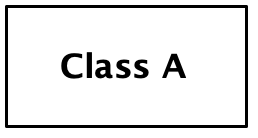
\includegraphics[width=0.5\textwidth]{diagrams/Conventions_Class.png}
        \caption{Rectangle shape.}
        \label{fig:diagram_conventions_rectangle}
    \end{subfigure}
    \qquad
    \centering
    \begin{subfigure}[b]{0.45\textwidth}
        \centering
        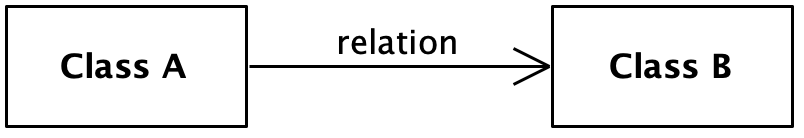
\includegraphics[width=\textwidth]{diagrams/Conventions_Relation.png}
        \caption{Labeled open arrow.}
        \label{fig:diagram_conventions_open_arrow}
    \end{subfigure}
    
    \centering
    \begin{subfigure}[b]{0.3\textwidth}
        \centering
        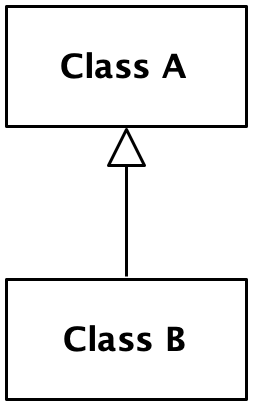
\includegraphics[width=0.5\textwidth]{diagrams/Conventions_Specialization.png}
        \caption{Closed arrow.}
        \label{fig:diagram_conventions_closed_arrow}
    \end{subfigure}
    \qquad
    \centering
    \begin{subfigure}[b]{0.35\textwidth}
        \centering
        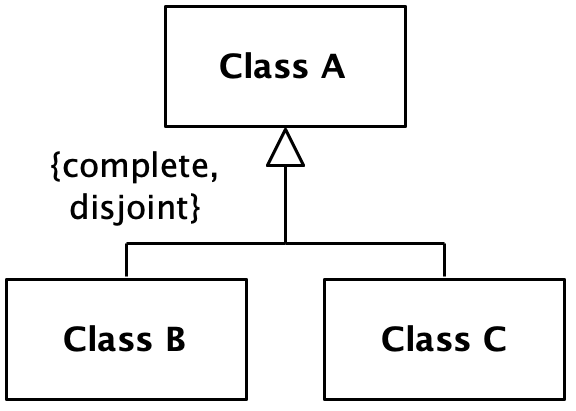
\includegraphics[width=\textwidth]{diagrams/Conventions_Generalization_Set.png}
        \caption{Labeled closed arrows.}
        \label{fig:diagram_conventions_labeled_arrow}
    \end{subfigure}
    \caption{UML-based representation of first-order logic axioms.}\label{fig:diagram_conventions}
\end{figure}

\begin{itemize}
    \item Rectangle shape (Figure~\ref{fig:diagram_conventions_rectangle}): visual representation of unary predicates associated to types in the ontology; the associated predicate is shown in lower camel case with no spaces.
    
    $classA(x)$

    \item Open arrow (Figure~\ref{fig:diagram_conventions_open_arrow}): visual representation of binary predicates; the predicate associated to the arrows' label is shown in lower camel case with no spaces; the predicate can only be true for any $x$ and $y$ if it is also true predicates associated to the types of each end (keeping the order of the arrow in the binary predicate's positions); this representation may also be associated to ternary predicates ifif its third position represents a time-index.
    
    $\forall x,y (relation(x,y) \rightarrow (classA(x) \wedge classB(y)))$
    
    $\forall x,y,w (relation(x,y,w) \rightarrow (classA(x) \wedge classB(y) \wedge world(w)))$

    \item Closed arrow (Figure~\ref{fig:diagram_conventions_closed_arrow}): visual representation of specializations between ontology's types, where the type in the tail of the arrow is a subtype of the type in the head of the arrow.
    
    $\forall x (classB(x) \rightarrow classA(x))$

    \item Labeled closed arrow (Figure~\ref{fig:diagram_conventions_labeled_arrow}): visual representation of disjoint and/or complete constraints over sets specializations between ontology's types.
    
    $\forall x (classB(x) \rightarrow classA(x))$\\
    $\forall x (classC(x) \rightarrow classA(x))$\\
    $\forall x (classA(x) \rightarrow (classB(x) \vee classC(x)))$  \hfill \{complete\}\\
    $\neg\exists x (classB(x) \wedge classC(x))$  \hfill \{disjoint\}
\end{itemize}

% 01_taxonomy_thing.p
\subsection{Partial Taxonomy of UFO: \me{Thing}}

This subsection presents most general types of UFO's taxonomy specializing the type \me{Thing} (Figure~\ref{fig:01_taxonomy_thing}).

\begin{figure}[ht]
    \centering
    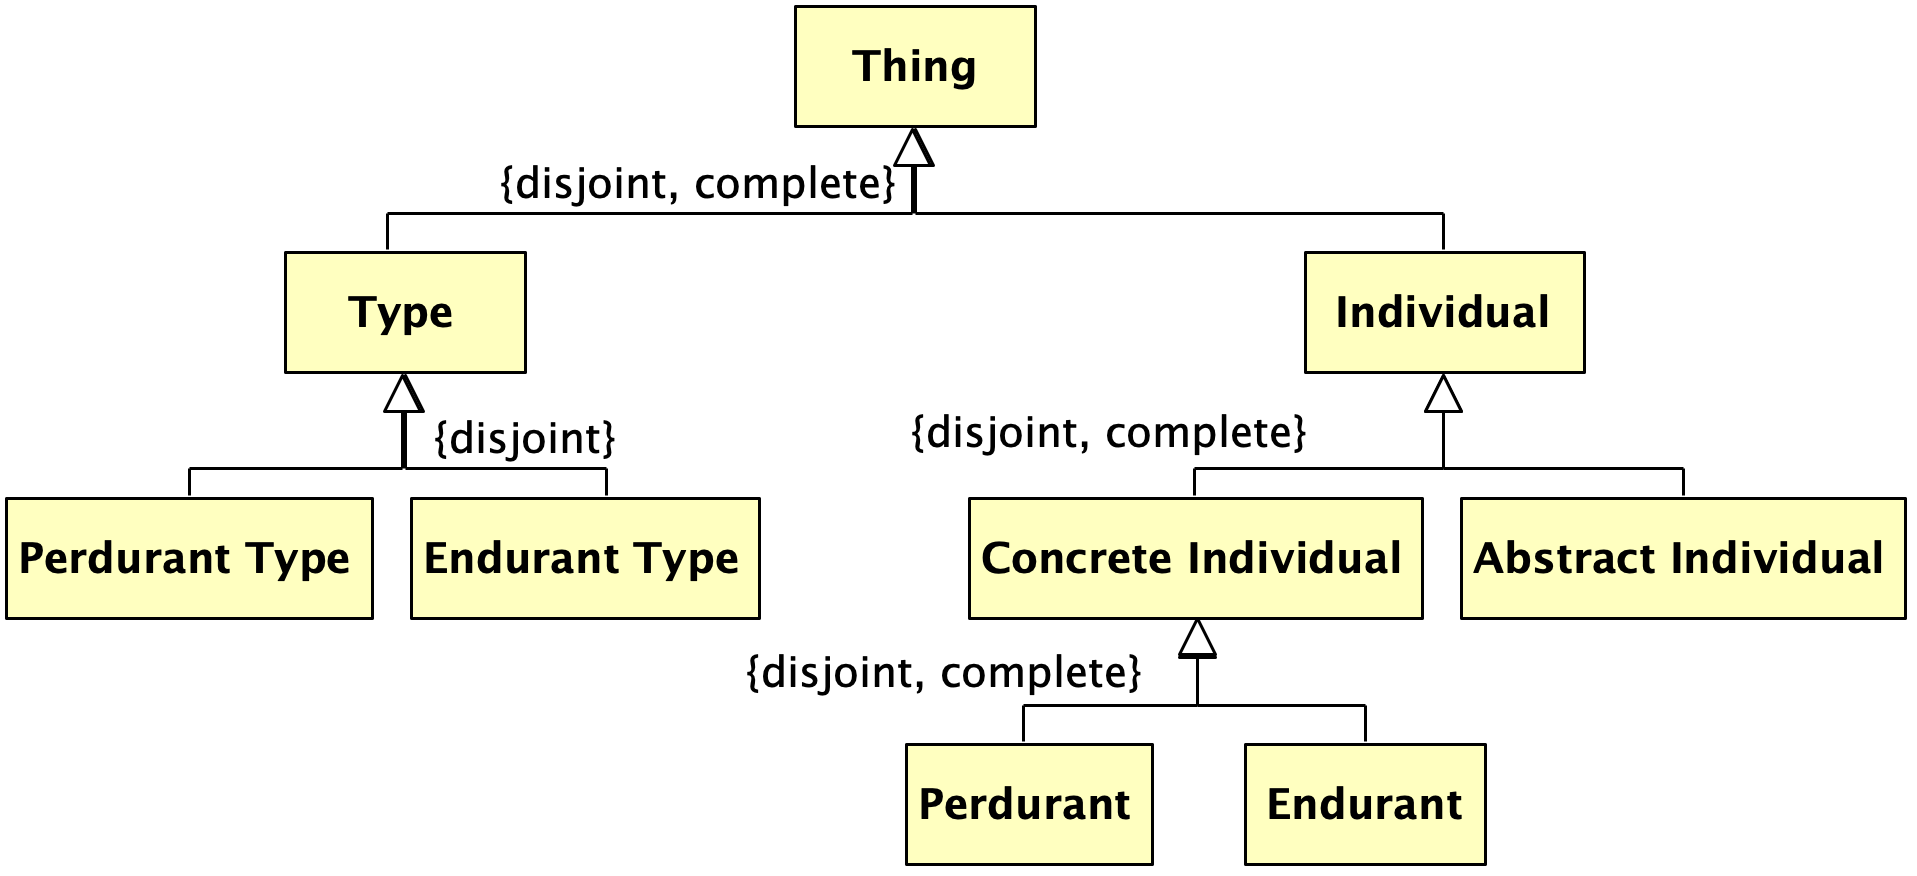
\includegraphics[width=0.8\textwidth]{diagrams/Thing_Diagram.png}
    \caption{Visual representation of UFO's taxonomy of \me{Thing}.}
    \label{fig:01_taxonomy_thing}
\end{figure}

\begin{itemize}
    \item[\myax{ax_thing_taxonomy}] For every $x$, $x$ is a \me{Thing} ifif $x$ is either a \me{Type} or an \me{Individual}.
    
    $\forall x(\textsf{type\_}(x)\vee \textsf{individual}(x)\leftrightarrow \textsf{thing}(x))$
    
    \lstinputlisting[firstline=1, lastline=6, firstnumber=1]{src/axioms-clif/01_taxonomy_thing.p.clif}
    
    
    \item[\myax{ax_thing_partition}] There is no $x$ such that it is a \me{Type} and an \me{Individual}.
    
    $\neg \exists x(\textsf{type\_}(x)\wedge \textsf{individual}(x))$
    
    \lstinputlisting[firstline=7, lastline=11, firstnumber=7]{src/axioms-clif/01_taxonomy_thing.p.clif}


    \item[\myax{ax_individual_taxonomy}] For every $x$, $x$ is an \me{Individual} ifif $x$ is either a \me{Concrete Individual} or an \me{Abstract Individual}.
    
    $\forall x(\textsf{concreteIndividual}(x)\vee \textsf{abstractIndividual}(x)\leftrightarrow \textsf{individual}(x))$

    \lstinputlisting[firstline=12, lastline=17, firstnumber=12]{src/axioms-clif/01_taxonomy_thing.p.clif}


    \item[\myax{ax_individual_partition}] There is no $x$ such that it is a \me{Concrete Individual} and an \me{Abstract Individual}.
    
    $\neg \exists x(\textsf{concreteIndividual}(x)\wedge \textsf{abstractIndividual}(x))$

    \lstinputlisting[firstline=18, lastline=22, firstnumber=18]{src/axioms-clif/01_taxonomy_thing.p.clif}

    
    \item[\myax{ax_concreteIndividual_taxonomy}] For every $x$, $x$ is a \me{Concrete Individual} ifif $x$ is either a \me{Perdurant} or an \me{Endurant}.
    
    $\forall x(\textsf{endurant}(x)\vee \textsf{perdurant}(x)\leftrightarrow \textsf{concreteIndividual}(x))$

    \lstinputlisting[firstline=23, lastline=28, firstnumber=23]{src/axioms-clif/01_taxonomy_thing.p.clif}


    \item[\myax{ax_concreteIndividual_partition}] There is no $x$ such that it is a \me{Perdurant} and an \me{Endurant}.
    
    $\neg \exists x(\textsf{endurant}(x)\wedge \textsf{perdurant}(x))$

    \lstinputlisting[firstline=29, lastline=33, firstnumber=29]{src/axioms-clif/01_taxonomy_thing.p.clif}

    
    \item[\myax{ax_type_taxonomy}] For every $x$, $x$ is a \me{Concrete Individual} ifif $x$ is either a \me{Perdurant} or an \me{Endurant}.
    
    $\forall x(\textsf{endurantType}(x)\vee \textsf{perdurantType}(x)\rightarrow \textsf{type\_}(x))$

    \lstinputlisting[firstline=34, lastline=39, firstnumber=34]{src/axioms-clif/01_taxonomy_thing.p.clif}


    \item[\myax{ax_type_partition}] There is no $x$ such that it is a \me{Perdurant Type} and an \me{Endurant Type}.
    
    $\neg \exists x(\textsf{endurantType}(x)\wedge \textsf{perdurantType}(x))$

    \lstinputlisting[firstline=40, lastline=44, firstnumber=40]{src/axioms-clif/01_taxonomy_thing.p.clif}
\end{itemize}



% 02_taxonomy_abstract_individual.p
\subsection{Partial Taxonomy of UFO: \me{Abstract Individual}}

This subsection presents a portion of UFO's taxonomy specializing the type \me{Abstract Individual} (Figure~\ref{fig:02_taxonomy_abstract_individual}).

\begin{figure}[ht]
    \centering
    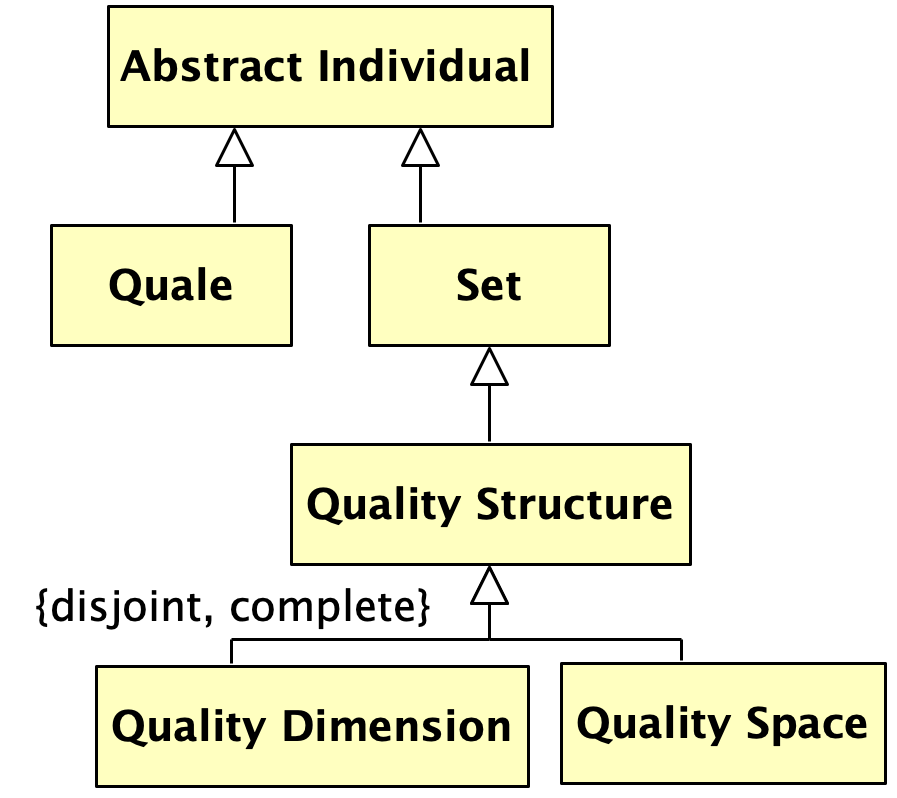
\includegraphics[width=0.4\textwidth]{diagrams/Abstract_Individual_Diagram.png}
    \caption{Visual representation of UFO's taxonomy of \me{Abstract Individual}.}
    \label{fig:02_taxonomy_abstract_individual}
\end{figure}

\begin{itemize}
    \item[\myax{ax_abstractIndividual_taxonomy_quale}] Every $x$ that is a \me{Quale} is also an \me{Abstract Individual}.
    
    $\forall x(\textsf{quale}(x)\rightarrow \textsf{abstractIndividual}(x))$
    
    \lstinputlisting[firstline=1, lastline=6, firstnumber=1]{src/axioms-clif/02_taxonomy_abstract_individual.p.clif}

    \item[\myax{ax_abstractIndividual_taxonomy_set}] Every $x$ that is a \me{Set} is also an \me{Abstract Individual}.
    
    $\forall x(\textsf{set\_}(x)\rightarrow \textsf{abstractIndividual}(x))$
    
    \lstinputlisting[firstline=7, lastline=12, firstnumber=7]{src/axioms-clif/02_taxonomy_abstract_individual.p.clif}

    \item[\myax{ax_abstractIndividual_taxonomy_world}] Every $x$ that is a \me{World} is also an \me{Abstract Individual}.
    
    $\forall x(\textsf{world}(x)\rightarrow \textsf{abstractIndividual}(x))$
    
    \lstinputlisting[firstline=13, lastline=18, firstnumber=13]{src/axioms-clif/02_taxonomy_abstract_individual.p.clif}

    \item[\myax{ax_abstractIndividual_pairwiseDisjoint}] There is no $x$ such that it is a \me{Quale}, a \me{Set}, and a \me{World} (pairwise disjoint).
    
    $\neg \exists x((\textsf{quale}(x)\wedge \textsf{set\_}(x))\vee (\textsf{quale}(x)\wedge \textsf{world}(x))\vee (\textsf{set\_}(x)\wedge \textsf{world}(x)))$
    
    \lstinputlisting[firstline=19, lastline=23, firstnumber=19]{src/axioms-clif/02_taxonomy_abstract_individual.p.clif}

    \item[\myax{ax_set_taxonomy_qualityStructure}] Every $x$ that is a \me{Quality Structure} is also a \me{Set}.
    
    $\forall x(\textsf{qualityStructure}(x)\rightarrow \textsf{set\_}(x))$
    
    \lstinputlisting[firstline=24, lastline=29, firstnumber=24]{src/axioms-clif/02_taxonomy_abstract_individual.p.clif}

    \item[\myax{ax_qualityStructure_taxonomy}] For every $x$, $x$ is a \me{Quality Structure} ifif $x$ is either a \me{Quality Dimension} or a \me{Quality Space}.
    
    $\forall x(\textsf{qualityDimension}(x)\vee \textsf{qualitySpace}(x)\leftrightarrow \textsf{qualityStructure}(x))$
    
    \lstinputlisting[firstline=30, lastline=35, firstnumber=30]{src/axioms-clif/02_taxonomy_abstract_individual.p.clif}
    
    
    \item[\myax{ax_qualityStructure_partition}] There is no $x$ such that it is a \me{Quality Dimension} and a \me{Quality Space}.
    
    $\neg \exists x(\textsf{qualityDimension}(x)\wedge \textsf{qualitySpace}(x))$
    
    \lstinputlisting[firstline=36, lastline=40, firstnumber=36]{src/axioms-clif/02_taxonomy_abstract_individual.p.clif}
\end{itemize}



% 03_taxonomy_endurant.p
\subsection{Partial Taxonomy of UFO: \me{Endurant}}

This subsection presents a portion of UFO's taxonomy specializing the type \me{Endurant} (Figure~\ref{fig:03_taxonomy_endurant}).

\begin{figure}[ht]
    \centering
    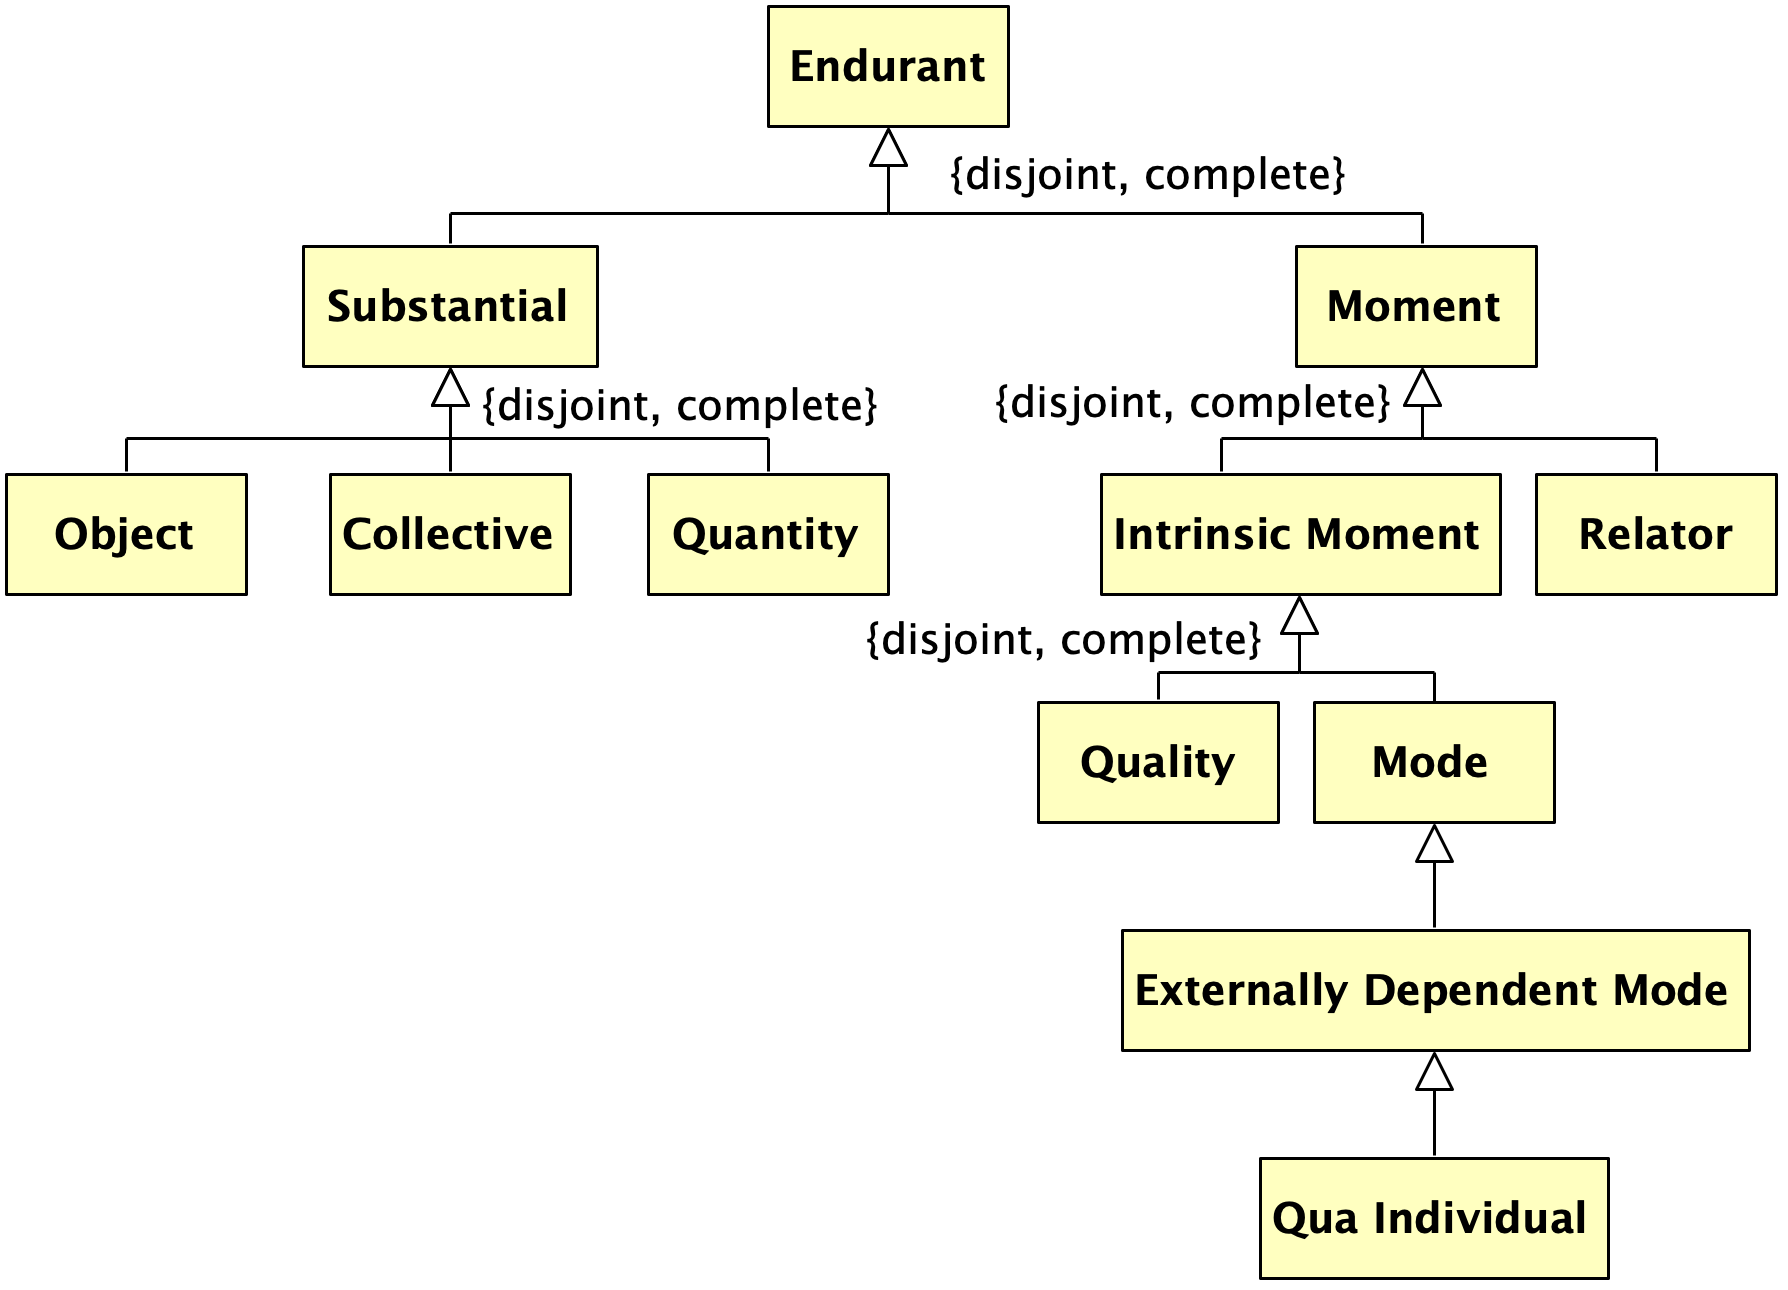
\includegraphics[width=0.8\textwidth]{diagrams/Endurant_Diagram.png}
    \caption{Visual representation of UFO's taxonomy of \me{Endurant}.}
    \label{fig:03_taxonomy_endurant}
\end{figure}

\begin{itemize}
    \item[\myax{ax_endurant_taxonomy}] For every $x$, $x$ is an \me{Endurant} ifif $x$ is either a \me{Substantial} or a \me{Moment}.
    
    $\forall x(\textsf{substantial}(x)\vee \textsf{moment}(x)\leftrightarrow \textsf{endurant}(x))$
    
    \lstinputlisting[firstline=1, lastline=6, firstnumber=1]{src/axioms-clif/03_taxonomy_endurant.p.clif}
    
    \item[\myax{ax_endurant_partition}] There is no $x$ such that it is a \me{Substantial} and a \me{Moment}.
    
    $\neg \exists x(\textsf{substantial}(x)\wedge \textsf{moment}(x))$
    
    \lstinputlisting[firstline=7, lastline=11, firstnumber=7]{src/axioms-clif/03_taxonomy_endurant.p.clif}
    
    \item[\myax{ax_substantial_taxonomy}] For every $x$, $x$ is a \me{Substantial} ifif $x$ is either an \me{Object}, a \me{Collective}, or a \me{Quantity}.
    
    $\forall x(\textsf{object}(x)\vee \textsf{collective}(x)\vee \textsf{quantity}(x)\leftrightarrow \textsf{substantial}(x))$
    
    \lstinputlisting[firstline=12, lastline=17, firstnumber=12]{src/axioms-clif/03_taxonomy_endurant.p.clif}
    
    \item[\myax{ax_substantial_partition}] There is no $x$ such that it is an \me{Object}, a \me{Collective}, and a \me{Quantity} (pairwise disjoint).
    
    $\neg \exists x((\textsf{object}(x)\wedge \textsf{collective}(x))\vee (\textsf{object}(x)\wedge \textsf{quantity}(x))\vee (\textsf{collective}(x)\wedge \textsf{quantity}(x)))$
    
    \lstinputlisting[firstline=18, lastline=22, firstnumber=18]{src/axioms-clif/03_taxonomy_endurant.p.clif}

    \item[\myax{ax_moment_taxonomy}] For every $x$, $x$ is a \me{Moment} ifif $x$ is either an \me{Intrinsic Moment} or a \me{Relator}.
    
    $\forall x(\textsf{intrinsicMoment}(x)\vee \textsf{relator}(x)\leftrightarrow \textsf{moment}(x))$
    
    \lstinputlisting[firstline=23, lastline=28, firstnumber=23]{src/axioms-clif/03_taxonomy_endurant.p.clif}
    
    \item[\myax{ax_moment_partition}] There is no $x$ such that it is an \me{Intrinsic Moment} and a \me{Relator}.
    
    $\neg \exists x(\textsf{intrinsicMoment}(x)\wedge \textsf{relator}(x))$
    
    \lstinputlisting[firstline=29, lastline=33, firstnumber=29]{src/axioms-clif/03_taxonomy_endurant.p.clif}

    \item[\myax{ax_intrinsicMoment_taxonomy}] For every $x$, $x$ is an \me{Intrinsic Moment} ifif $x$ is either a \me{Quality} or a \me{Mode}.
    
    $\forall x(\textsf{quality}(x)\vee \textsf{mode}(x)\leftrightarrow \textsf{intrinsicMoment}(x))$
    
    \lstinputlisting[firstline=34, lastline=39, firstnumber=34]{src/axioms-clif/03_taxonomy_endurant.p.clif}
    
    
    \item[\myax{ax_intrinsicMoment_partition}] There is no $x$ such that it is an \me{Intrinsic Moment} and a \me{Relator}.
    
    $\neg \exists x(\textsf{quality}(x)\wedge \textsf{mode}(x))$
    
    \lstinputlisting[firstline=40, lastline=44, firstnumber=40]{src/axioms-clif/03_taxonomy_endurant.p.clif}

    \item[\myax{ax_mode_taxonomy_disposition}] Every $x$ that is a \me{Disposition} is also a \me{Mode}.
    
    $\forall x(\textsf{disposition}(x)\rightarrow \textsf{mode}(x))$
    
    \lstinputlisting[firstline=45, lastline=50, firstnumber=45]{src/axioms-clif/03_taxonomy_endurant.p.clif}

    \item[\myax{ax_mode_taxonomy_externallyDependentMode}] Every $x$ that is an \me{Externally Dependent Mode} is also a \me{Mode}.
    
    $\forall x(\textsf{externallyDependentMode}(x)\rightarrow \textsf{mode}(x))$
    
    \lstinputlisting[firstline=51, lastline=56, firstnumber=51]{src/axioms-clif/03_taxonomy_endurant.p.clif}

    \item[\myax{ax_externallyDependentMode_taxonomy_quaIndividual}] Every $x$ that is an \me{Qua Individual} is also an \me{Externally Dependent Mode}.
    
    $\forall x(\textsf{quaIndividual}(x)\rightarrow \textsf{externallyDependentMode}(x))$
    
    \lstinputlisting[firstline=57, lastline=62, firstnumber=57]{src/axioms-clif/03_taxonomy_endurant.p.clif}
\end{itemize}



% 04_taxonomy_endurant_type_nature.p
\subsection{Partial Taxonomy of UFO: \me{Endurant Type} by Ontological Natures}

This subsection presents a portion of UFO's taxonomy specializing the type \me{Endurant Type} classified by ontological natures (Figure~\ref{fig:04_taxonomy_endurant_type_nature}).

\begin{figure}[ht]
    \centering
    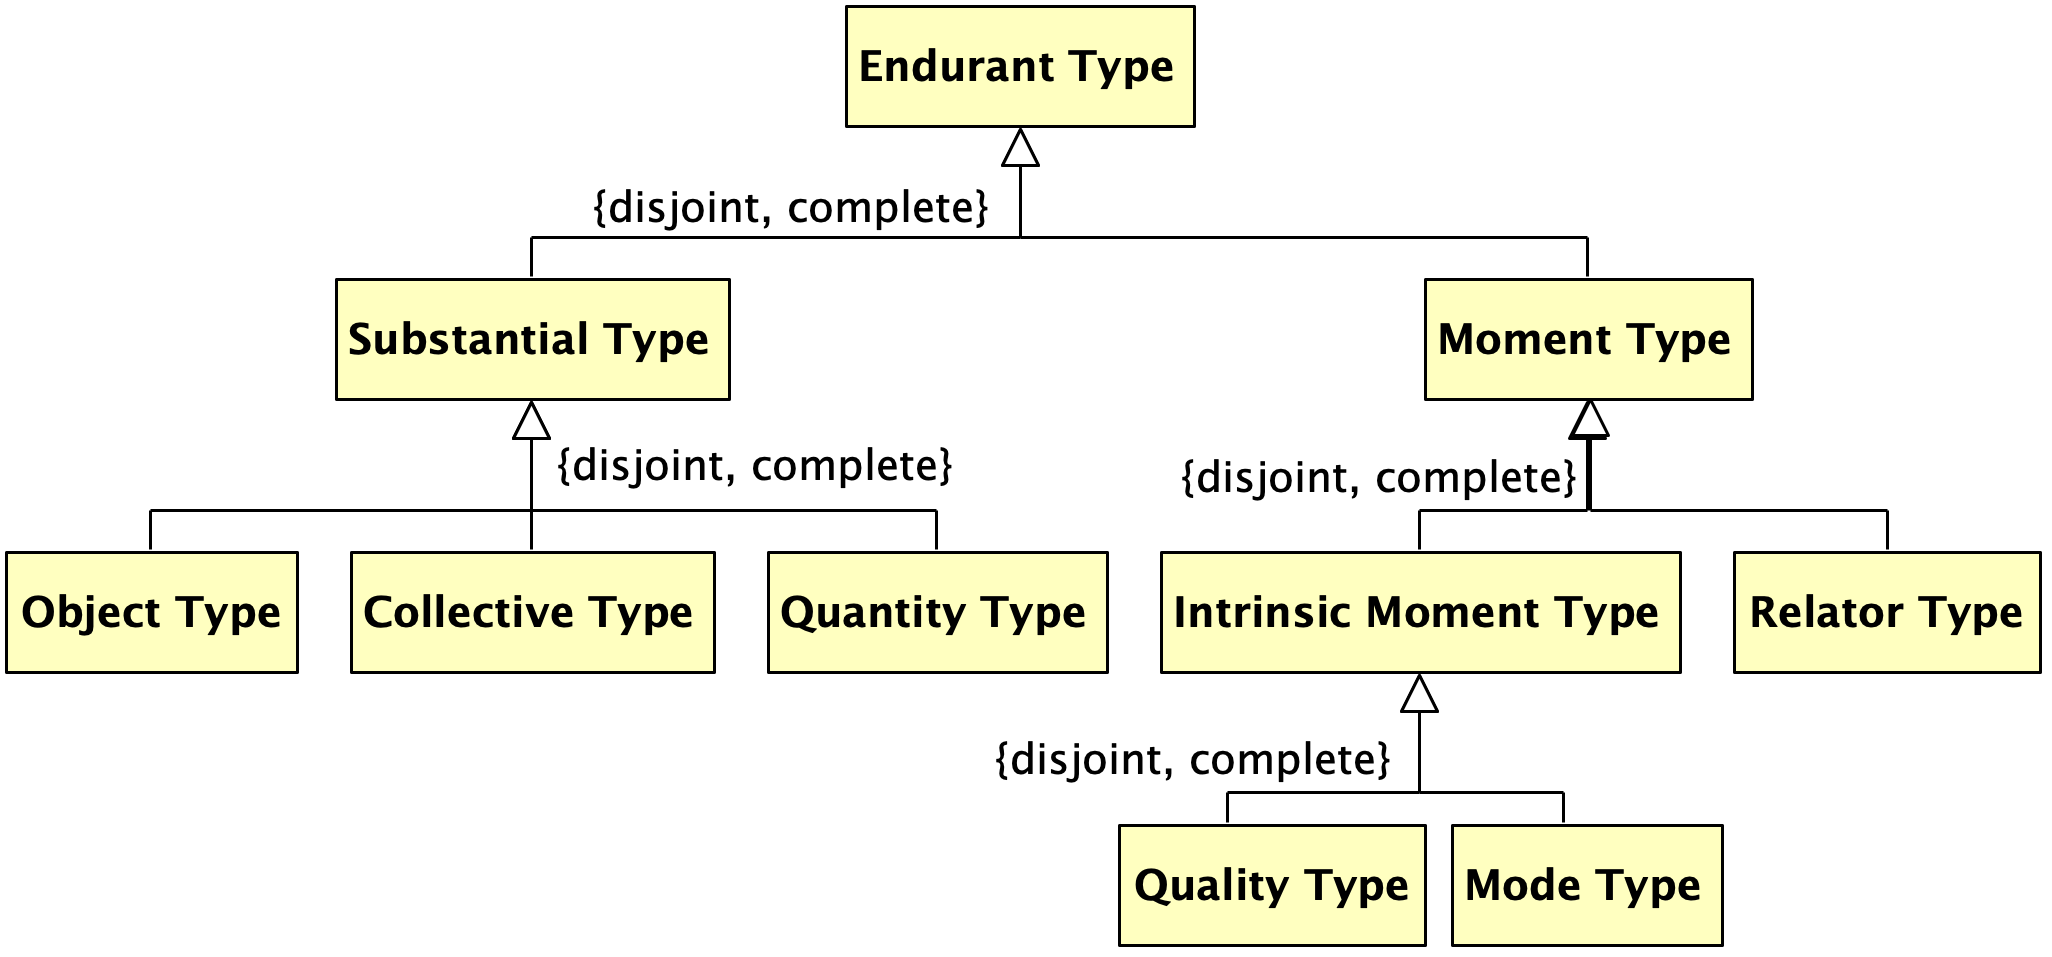
\includegraphics[width=0.9\textwidth]{diagrams/Endurant_Type_Natures_Diagram.png}
    \caption{Visual representation of UFO's taxonomy of \me{Endurant Type} classified by ontological natures.}
    \label{fig:04_taxonomy_endurant_type_nature}
\end{figure}

\begin{itemize}
    \item[\myax{ax_endurantType_taxonomy_nature}] For every $x$, $x$ is an \me{Endurant Type} ifif $x$ is either a \me{Substantial Type} or a \me{Moment Type}.
    
    $\forall x(\textsf{substantialType}(x)\vee \textsf{momentType}(x)\leftrightarrow \textsf{endurantType}(x))$
    
    \lstinputlisting[firstline=1, lastline=6, firstnumber=1]{src/axioms-clif/04_taxonomy_endurant_type_nature.p.clif}
    
    \item[\myax{ax_endurantType_partition_nature}] There is no $x$ such that it is a \me{Substantial Type} and a \me{Moment Type}.
    
    $\neg \exists x(\textsf{substantialType}(x)\wedge \textsf{momentType}(x))$
    
    \lstinputlisting[firstline=7, lastline=11, firstnumber=7]{src/axioms-clif/04_taxonomy_endurant_type_nature.p.clif}

    \item[\myax{ax_substantialType_taxonomy}] For every $x$, $x$ is a \me{Substantial Type} ifif $x$ is either an \me{Object Type}, a \me{Collective Type}, or a \me{Quantity Type}.
    
    $\forall x(\textsf{objectType}(x)\vee \textsf{collectiveType}(x)\vee \textsf{quantityType}(x)\leftrightarrow \textsf{substantialType}(x))$
    
    \lstinputlisting[firstline=12, lastline=17, firstnumber=12]{src/axioms-clif/04_taxonomy_endurant_type_nature.p.clif}
    
    \item[\myax{ax_substantialType_partition}] There is no $x$ such that it is an \me{Object Type}, a \me{Collective Type}, and a \me{Quantity Type} (pairwise disjoint).
    
    $\neg \exists x((\textsf{objectType}(x)\wedge \textsf{collectiveType}(x))\vee (\textsf{objectType}(x)\wedge \textsf{quantityType}(x))\vee (\textsf{collectiveType}(x)\wedge \textsf{quantityType}(x)))$
    
    \lstinputlisting[firstline=18, lastline=22, firstnumber=18]{src/axioms-clif/04_taxonomy_endurant_type_nature.p.clif}

    \item[\myax{ax_momentType_taxonomy}] For every $x$, $x$ is a \me{Moment Type} ifif $x$ is either an \me{Intrinsic Moment Type} or a \me{Relator Type}.
    
    $\forall x(\textsf{intrinsicMomentType}(x)\vee \textsf{relatorType}(x)\leftrightarrow \textsf{momentType}(x))$
    
    \lstinputlisting[firstline=23, lastline=28, firstnumber=23]{src/axioms-clif/04_taxonomy_endurant_type_nature.p.clif}
    
    \item[\myax{ax_momentType_partition}] There is no $x$ such that it is an \me{Intrinsic Moment Type} and a \me{Relator Type}.
    
    $\neg \exists x(\textsf{intrinsicMomentType}(x)\wedge \textsf{relatorType}(x))$
    
    \lstinputlisting[firstline=29, lastline=33, firstnumber=29]{src/axioms-clif/04_taxonomy_endurant_type_nature.p.clif}

    \item[\myax{ax_intrinsicMomentType_taxonomy}] For every $x$, $x$ is an \me{Intrinsic Moment Type} ifif $x$ is either a \me{Quality Type} or a \me{Mode Type}.
    
    $\forall x(\textsf{qualityType}(x)\vee \textsf{modeType}(x)\leftrightarrow \textsf{intrinsicMomentType}(x))$
    
    \lstinputlisting[firstline=34, lastline=39, firstnumber=34]{src/axioms-clif/04_taxonomy_endurant_type_nature.p.clif}
    
    \item[\myax{ax_intrinsicMomentType_partition}] There is no $x$ such that it is an \me{Intrinsic Moment Type} and a \me{Relator Type}.
    
    $\neg \exists x(\textsf{qualityType}(x)\wedge \textsf{modeType}(x))$
    
    \lstinputlisting[firstline=40, lastline=44, firstnumber=40]{src/axioms-clif/04_taxonomy_endurant_type_nature.p.clif}
\end{itemize}



% 05_taxonomy_endurant_types_properties.p
\subsection{Partial Taxonomy of UFO: \me{Endurant Type} by Modal Properties of Types}

This subsection presents a portion of UFO's taxonomy specializing the type \me{Endurant Type} classified by the modal properties of types (Figure~\ref{fig:05_taxonomy_endurant_types_properties}).

\begin{figure}[ht]
    \centering
    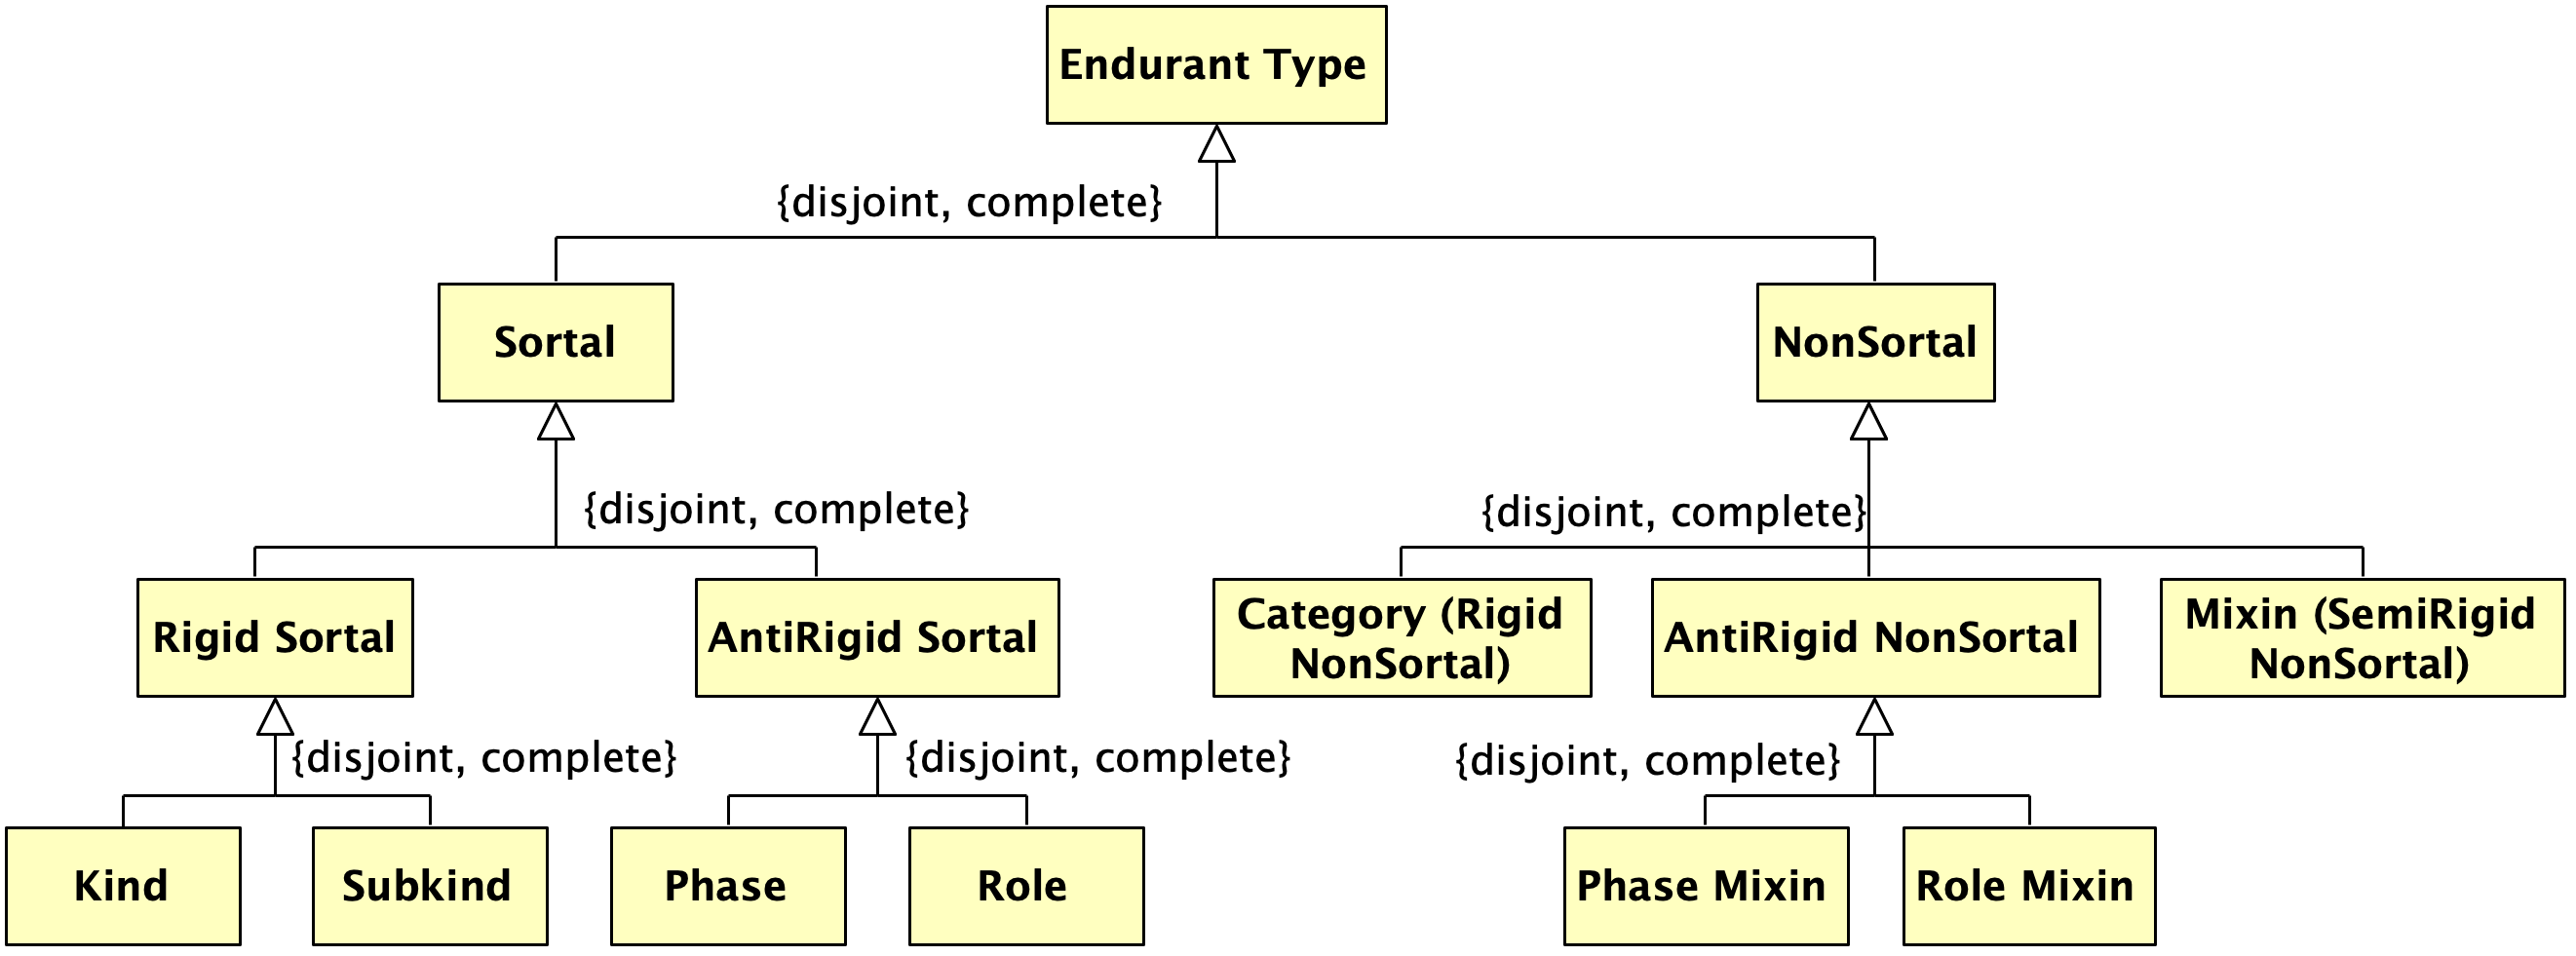
\includegraphics[width=\textwidth]{diagrams/Endurant_Type_Properties_Diagram.png}
    \caption{Visual representation of UFO's taxonomy of \me{Endurant Type} classified by the modal properties of types.}
    \label{fig:05_taxonomy_endurant_types_properties}
\end{figure}

\begin{itemize}
    \item[\myax{ax_endurantType_taxonomy_properties}] For every $x$, $x$ is an \me{Endurant Type} ifif $x$ is either a \me{Sortal} or a \me{NonSortal}.
    
    $\forall x(\textsf{sortal}(x)\vee \textsf{nonSortal}(x)\leftrightarrow \textsf{endurantType}(x))$
    
    \lstinputlisting[firstline=1, lastline=6, firstnumber=1]{src/axioms-clif/05_taxonomy_endurant_types_properties.p.clif}
    
    \item[\myax{ax_endurantType_partition_properties}] There is no $x$ such that it is a \me{Sortal} and a \me{NonSortal}.
    
    $\neg \exists x(\textsf{sortal}(x)\wedge \textsf{nonSortal}(x))$
    
    \lstinputlisting[firstline=7, lastline=11, firstnumber=7]{src/axioms-clif/05_taxonomy_endurant_types_properties.p.clif}

    \item[\myax{ax_sortal_taxonomy}] For every $x$, $x$ is a \me{Sortal} ifif $x$ is either a \me{Rigid Sortal} or an \me{AntiRigid Sortal}.
    
    $\forall x(\textsf{rigidSortal}(x)\vee \textsf{antiRigidSortal}(x)\leftrightarrow \textsf{sortal}(x))$
    
    \lstinputlisting[firstline=12, lastline=17, firstnumber=12]{src/axioms-clif/05_taxonomy_endurant_types_properties.p.clif}
    
    \item[\myax{ax_sortal_partition}] There is no $x$ such that it is a \me{Rigid Sortal} and an \me{AntiRigid Sortal}.
    
    $\neg \exists x(\textsf{rigidSortal}(x)\wedge \textsf{antiRigidSortal}(x))$
    
    \lstinputlisting[firstline=18, lastline=22, firstnumber=18]{src/axioms-clif/05_taxonomy_endurant_types_properties.p.clif}

    \item[\myax{ax_rigidSortal_taxonomy}] For every $x$, $x$ is a \me{Rigid Sortal} ifif $x$ is either a \me{Kind} or a \me{Subkind}.
    
    $\forall x(\textsf{kind}(x)\vee \textsf{subkind}(x)\leftrightarrow \textsf{rigidSortal}(x))$
    
    \lstinputlisting[firstline=23, lastline=28, firstnumber=23]{src/axioms-clif/05_taxonomy_endurant_types_properties.p.clif}
    
    \item[\myax{ax_rigidSortal_partition}] There is no $x$ such that it is a \me{Kind} and a \me{Subkind}.
    
    $\neg \exists x(\textsf{kind}(x)\wedge \textsf{subkind}(x))$
    
    \lstinputlisting[firstline=29, lastline=33, firstnumber=29]{src/axioms-clif/05_taxonomy_endurant_types_properties.p.clif}

    \item[\myax{ax_antiRigidSortal_taxonomy}] For every $x$, $x$ is an \me{AntiRigid Sortal} ifif $x$ is either a \me{Phase} or a \me{Role}.
    
    $\forall x(\textsf{phase}(x)\vee \textsf{role}(x)\leftrightarrow \textsf{antiRigidSortal}(x))$
    
    \lstinputlisting[firstline=34, lastline=39, firstnumber=34]{src/axioms-clif/05_taxonomy_endurant_types_properties.p.clif}
    
    \item[\myax{ax_antiRigidSortal_partition}] There is no $x$ such that it is a \me{Phase} and a \me{Role}.
    
    $\neg \exists x(\textsf{phase}(x)\wedge \textsf{role}(x))$
    
    \lstinputlisting[firstline=40, lastline=44, firstnumber=40]{src/axioms-clif/05_taxonomy_endurant_types_properties.p.clif}

    \item[\myax{ax_nonSortal_taxonomy}] For every $x$, $x$ is a \me{NonSortal} ifif $x$ is either a \me{Rigid NonSortal}, an \me{AntiRigid NonSortal}, or a \me{SemmiRigid NonSortal}.
    
    $\forall x(\textsf{rigidNonSortal}(x)\vee \textsf{semiRigidNonSortal}(x)\vee \textsf{antiRigidNonSortal}(x)\leftrightarrow \textsf{nonSortal}(x))$
    
    \lstinputlisting[firstline=45, lastline=50, firstnumber=45]{src/axioms-clif/05_taxonomy_endurant_types_properties.p.clif}
    
    \item[\myax{ax_nonSortal_partition}] There is no $x$ such that it is an \me{Rigid NonSortal}, an \me{AntiRigid NonSortal}, and a \me{SemiRigid NonSortal} (pairwise disjoint). 
    
    $\neg \exists x((\textsf{rigidNonSortal}(x)\wedge \textsf{semiRigidNonSortal}(x))\vee (\textsf{rigidNonSortal}(x)\wedge \textsf{antiRigidNonSortal}(x))\vee (\textsf{semiRigidNonSortal}(x)\wedge \textsf{antiRigidNonSortal}(x)))$
    
    \lstinputlisting[firstline=51, lastline=55, firstnumber=51]{src/axioms-clif/05_taxonomy_endurant_types_properties.p.clif}

    \item[\myax{ax_rigidNonSortal_taxonomy}] Every $x$ that is a \me{Rigid NonSortal} is also a \me{Category}.
    
    $\forall x(\textsf{rigidNonSortal}(x)\leftrightarrow \textsf{category}(x))$
    
    \lstinputlisting[firstline=56, lastline=61, firstnumber=56]{src/axioms-clif/05_taxonomy_endurant_types_properties.p.clif}

    \item[\myax{ax_semiRigidNonSortal_taxonomy}] Every $x$ that is a \me{SemiRigid NonSortal} is also a \me{Mixin}.
    
    $\forall x(\textsf{semiRigidNonSortal}(x)\leftrightarrow \textsf{mixin}(x))$
    
    \lstinputlisting[firstline=62, lastline=67, firstnumber=62]{src/axioms-clif/05_taxonomy_endurant_types_properties.p.clif}

    \item[\myax{ax_antiRigidNonSortal_taxonomy}] For every $x$, $x$ is an \me{AntiRigid NonSortal} ifif $x$ is either a \me{Phase Mixin} or a \me{Role Mixin}.
    
    $\forall x(\textsf{phaseMixin}(x)\vee \textsf{roleMixin}(x)\leftrightarrow \textsf{antiRigidNonSortal}(x))$
    
    \lstinputlisting[firstline=68, lastline=73, firstnumber=68]{src/axioms-clif/05_taxonomy_endurant_types_properties.p.clif}
    
    \item[\myax{ax_antiRigidNonSortal_partition}] There is no $x$ such that it is a \me{Phase Mixin} and a \me{Role Mixin}.
    
    $\neg \exists x(\textsf{phaseMixin}(x)\wedge \textsf{roleMixin}(x))$
    
    \lstinputlisting[firstline=74, lastline=78, firstnumber=74]{src/axioms-clif/05_taxonomy_endurant_types_properties.p.clif}
\end{itemize}




% ------------------------------ BEGIN DEPRECATED ------------------------------


% \subsection{UFO Taxonomy}

% % Types, Individuals, Instantiation, and Specialization
% \subsubsection{Defining Types, Individuals, and Specialization}

% \begin{figure}[ht]
%     \centering
%     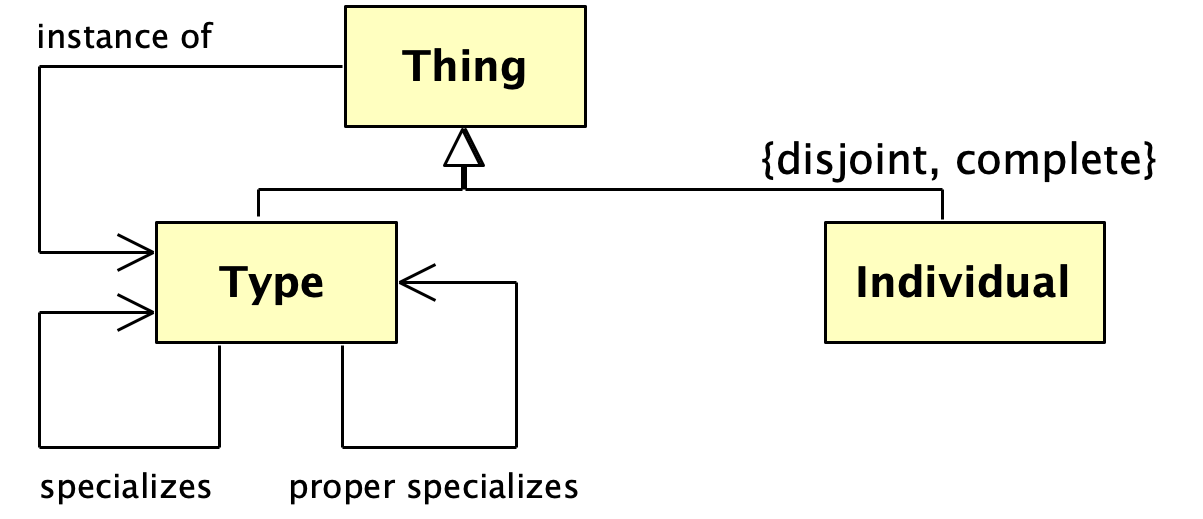
\includegraphics[width=0.6\textwidth]{diagrams/Instantiation_Diagram.png}
%     \caption{Types, individuals, instantiation, and specialization.}
%     \label{fig:instantiation_and_specialization}
% \end{figure}

% \lstinputlisting[
%     firstline=\BeginInstantationAndSpecialzation, 
%     lastline=\EndInstantationAndSpecialzation, 
%     firstnumber=\BeginInstantationAndSpecialzation
% ]{ufo_2021.tex}

% % Sortality and Rigidity
% \subsubsection{Defining Rigidity and Sortality}

% \lstinputlisting[
%     firstline=\BeginRigidityAndSortality, 
%     lastline=\EndRigidityAndSortality, 
%     firstnumber=\BeginRigidityAndSortality
% ]{ufo_2021.tex}

% % Endurant Types Definition
% \subsubsection{Defining Endurant Types}

% \lstinputlisting[
%     firstline=\BeginEndurantsTypesDefinition, 
%     lastline=\EndEndurantsTypesDefinition, 
%     firstnumber=\BeginEndurantsTypesDefinition
% ]{ufo_2021.tex}

% % Mereology
% \subsubsection{Mereology}

% \lstinputlisting[
%     firstline=\BeginMereology, 
%     lastline=\EndMereology, 
%     firstnumber=\BeginMereology
% ]{ufo_2021.tex}

% % Composition
% \subsubsection{Composition}

% \lstinputlisting[
%     firstline=\BeginComposition, 
%     lastline=\EndComposition, 
%     firstnumber=\BeginComposition
% ]{ufo_2021.tex}

% % Constitution
% \subsubsection{Constitution}

% \lstinputlisting[
%     firstline=\BeginConstitution, 
%     lastline=\EndConstitution, 
%     firstnumber=\BeginConstitution
% ]{ufo_2021.tex}

% % Existential Dependence
% \subsubsection{Existential Dependence}

% \lstinputlisting[
%     firstline=\BeginExistentialDependence, 
%     lastline=\EndExistentialDependence, 
%     firstnumber=\BeginExistentialDependence
% ]{ufo_2021.tex}

% % Moments and Inherence
% \subsubsection{Moments and Inherence}

% \lstinputlisting[
%     firstline=\BeginMomentsAndInherence, 
%     lastline=\EndMomentsAndInherence, 
%     firstnumber=\BeginMomentsAndInherence
% ]{ufo_2021.tex}

% % Relators
% \subsubsection{Relators}

% \lstinputlisting[
%     firstline=\BeginRelators, 
%     lastline=\EndRelators, 
%     firstnumber=\BeginRelators
% ]{ufo_2021.tex}

% % Characterization
% \subsubsection{Characterization}

% \lstinputlisting[
%     firstline=\BeginCharacterization, 
%     lastline=\EndCharacterization, 
%     firstnumber=\BeginCharacterization
% ]{ufo_2021.tex}

% % Qualities and Quality Structures
% \subsubsection{Qualities and Quality Structures}

% \lstinputlisting[
%     firstline=\BeginQualitiesAndQualityStructures, 
%     lastline=\EndQualitiesAndQualityStructures, 
%     firstnumber=\BeginQualitiesAndQualityStructures
% ]{ufo_2021.tex}

% % Endurants and Perdurants
% \subsubsection{Endurants and Perdurants}

% \lstinputlisting[
%     firstline=\BeginEndurantsAndPerdurants, 
%     lastline=\EndEndurantsAndPerdurants, 
%     firstnumber=\BeginEndurantsAndPerdurants
% ]{ufo_2021.tex}

% \bibliographystyle{abbrv}
% \bibliography{main}

\end{document}